\chapter{پرسش‌های بازه‌ای}

\index{range query@پرسش بازه‌ای}
\index{sum query@پرسش مجموع}
\index{minimum query@پرسش کمینه}
\index{maximum query@پرسش بیشینه}

در این فصل داده‌ساختارهایی بررسی می‌شوند
که پردازش کارآمد پرسش‌های بازه‌ای را ممکن می‌سازند.
در یک \key{پرسش بازه‌ای}،
هدف محاسبه یک مقدار
بر اساس زیرآرایه‌ای از یک آرایه است.
پرسش‌های بازه‌ای متداول عبارتند از:
\begin{itemize}
\item $\texttt{sum}_q(a,b)$: محاسبه مجموع مقادیر در بازه $[a,b]$
\item $\texttt{min}_q(a,b)$: یافتن مقدار کمینه در بازه $[a,b]$
\item $\texttt{max}_q(a,b)$: یافتن مقدار بیشینه در بازه $[a,b]$
\end{itemize}

برای مثال، بازه $[3,6]$ در آرایه زیر را در نظر بگیرید:
\begin{center}
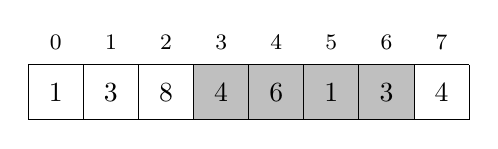
\begin{tikzpicture}[scale=0.7]
\fill[color=lightgray] (3,0) rectangle (7,1);
\draw (0,0) grid (8,1);

\node at (0.5,0.5) {$1$};
\node at (1.5,0.5) {$3$};
\node at (2.5,0.5) {$8$};
\node at (3.5,0.5) {$4$};
\node at (4.5,0.5) {$6$};
\node at (5.5,0.5) {$1$};
\node at (6.5,0.5) {$3$};
\node at (7.5,0.5) {$4$};

\footnotesize
\node at (0.5,1.4) {$0$};
\node at (1.5,1.4) {$1$};
\node at (2.5,1.4) {$2$};
\node at (3.5,1.4) {$3$};
\node at (4.5,1.4) {$4$};
\node at (5.5,1.4) {$5$};
\node at (6.5,1.4) {$6$};
\node at (7.5,1.4) {$7$};
\end{tikzpicture}
\end{center}
در این حالت، $\texttt{sum}_q(3,6)=14$،
$\texttt{min}_q(3,6)=1$ و $\texttt{max}_q(3,6)=6$ است.

روشی ساده برای پردازش پرسش‌های بازه‌ای استفاده از
حلقه‌ای است که تمام مقادیر آرایه در بازه را پیمایش می‌کند.
برای نمونه، تابع زیر می‌تواند
برای پردازش پرسش‌های مجموع روی آرایه استفاده شود:

\begin{lstlisting}
int sum(int a, int b) {
    int s = 0;
    for (int i = a; i <= b; i++) {
        s += array[i];
    }
    return s;
}
\end{lstlisting}

این تابع در زمان $O(n)$ اجرا می‌شود،
که $n$ اندازه آرایه است.
بنابراین با این تابع می‌توان $q$ پرسش را در زمان $O(nq)$
پردازش کرد.
اما اگر $n$ و $q$ بزرگ باشند، این روش
کند است. روش‌هایی وجود دارند که
پرسش‌های بازه‌ای را بسیار کارآمدتر پردازش می‌کنند.

\section{پرسش‌های آرایه ایستا}

ابتدا حالتی بررسی می‌شود که
آرایه \emph{ایستا} است؛ یعنی
مقادیر آرایه هرگز بین پرسش‌ها به‌روزرسانی نمی‌شوند.
در این حالت ساختن داده‌ساختاری ایستا
که پاسخ هر پرسش ممکن را بدهد کافی است.

\subsubsection{پرسش‌های مجموع}

\index{prefix sum array@آرایه مجموع پیشوندی}

پرسش‌های مجموع روی آرایه ایستا
با ساخت یک \key{آرایه مجموع پیشوندی} به سادگی پردازش می‌شوند.
هر مقدار در آرایه مجموع پیشوندی برابر با
مجموع مقادیر در آرایه اصلی تا آن جایگاه است؛
یعنی مقدار در جایگاه $k$ برابر با $\texttt{sum}_q(0,k)$ است.
آرایه مجموع پیشوندی در زمان $O(n)$ ساخته می‌شود.

برای مثال، آرایه زیر را در نظر بگیرید:
\begin{center}
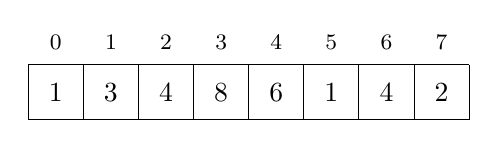
\begin{tikzpicture}[scale=0.7]
%\fill[color=lightgray] (3,0) rectangle (7,1);
\draw (0,0) grid (8,1);

\node at (0.5,0.5) {$1$};
\node at (1.5,0.5) {$3$};
\node at (2.5,0.5) {$4$};
\node at (3.5,0.5) {$8$};
\node at (4.5,0.5) {$6$};
\node at (5.5,0.5) {$1$};
\node at (6.5,0.5) {$4$};
\node at (7.5,0.5) {$2$};

\footnotesize
\node at (0.5,1.4) {$0$};
\node at (1.5,1.4) {$1$};
\node at (2.5,1.4) {$2$};
\node at (3.5,1.4) {$3$};
\node at (4.5,1.4) {$4$};
\node at (5.5,1.4) {$5$};
\node at (6.5,1.4) {$6$};
\node at (7.5,1.4) {$7$};
\end{tikzpicture}
\end{center}
آرایه مجموع پیشوندی متناظر به صورت زیر است:
\begin{center}
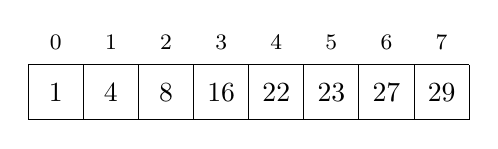
\begin{tikzpicture}[scale=0.7]
%\fill[color=lightgray] (3,0) rectangle (7,1);
\draw (0,0) grid (8,1);

\node at (0.5,0.5) {$1$};
\node at (1.5,0.5) {$4$};
\node at (2.5,0.5) {$8$};
\node at (3.5,0.5) {$16$};
\node at (4.5,0.5) {$22$};
\node at (5.5,0.5) {$23$};
\node at (6.5,0.5) {$27$};
\node at (7.5,0.5) {$29$};


\footnotesize
\node at (0.5,1.4) {$0$};
\node at (1.5,1.4) {$1$};
\node at (2.5,1.4) {$2$};
\node at (3.5,1.4) {$3$};
\node at (4.5,1.4) {$4$};
\node at (5.5,1.4) {$5$};
\node at (6.5,1.4) {$6$};
\node at (7.5,1.4) {$7$};
\end{tikzpicture}
\end{center}
از آنجا که آرایه مجموع پیشوندی شامل تمام مقادیر
$\texttt{sum}_q(0,k)$ است،
می‌توان هر مقدار از
$\texttt{sum}_q(a,b)$ را در زمان $O(1)$ به صورت زیر محاسبه کرد:
\[ \texttt{sum}_q(a,b) = \texttt{sum}_q(0,b) - \texttt{sum}_q(0,a-1)\]
با تعریف $\texttt{sum}_q(0,-1)=0$،
فرمول فوق برای حالت $a=0$ نیز برقرار است.

به عنوان مثال، بازه $[3,6]$ را در نظر بگیرید:
\begin{center}
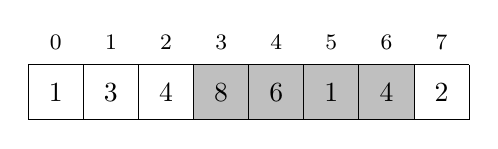
\begin{tikzpicture}[scale=0.7]
\fill[color=lightgray] (3,0) rectangle (7,1);
\draw (0,0) grid (8,1);

\node at (0.5,0.5) {$1$};
\node at (1.5,0.5) {$3$};
\node at (2.5,0.5) {$4$};
\node at (3.5,0.5) {$8$};
\node at (4.5,0.5) {$6$};
\node at (5.5,0.5) {$1$};
\node at (6.5,0.5) {$4$};
\node at (7.5,0.5) {$2$};

\footnotesize
\node at (0.5,1.4) {$0$};
\node at (1.5,1.4) {$1$};
\node at (2.5,1.4) {$2$};
\node at (3.5,1.4) {$3$};
\node at (4.5,1.4) {$4$};
\node at (5.5,1.4) {$5$};
\node at (6.5,1.4) {$6$};
\node at (7.5,1.4) {$7$};
\end{tikzpicture}
\end{center}
در این حالت $\texttt{sum}_q(3,6)=8+6+1+4=19$.
این مجموع را می‌توان از
دو مقدار آرایه مجموع پیشوندی به دست آورد:
\begin{center}
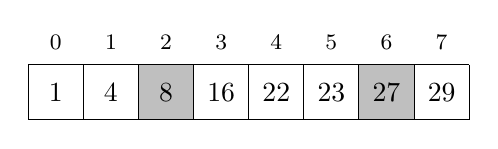
\begin{tikzpicture}[scale=0.7]
\fill[color=lightgray] (2,0) rectangle (3,1);
\fill[color=lightgray] (6,0) rectangle (7,1);
\draw (0,0) grid (8,1);

\node at (0.5,0.5) {$1$};
\node at (1.5,0.5) {$4$};
\node at (2.5,0.5) {$8$};
\node at (3.5,0.5) {$16$};
\node at (4.5,0.5) {$22$};
\node at (5.5,0.5) {$23$};
\node at (6.5,0.5) {$27$};
\node at (7.5,0.5) {$29$};

\footnotesize
\node at (0.5,1.4) {$0$};
\node at (1.5,1.4) {$1$};
\node at (2.5,1.4) {$2$};
\node at (3.5,1.4) {$3$};
\node at (4.5,1.4) {$4$};
\node at (5.5,1.4) {$5$};
\node at (6.5,1.4) {$6$};
\node at (7.5,1.4) {$7$};
\end{tikzpicture}
\end{center}
بنابراین، $\texttt{sum}_q(3,6)=\texttt{sum}_q(0,6)-\texttt{sum}_q(0,2)=27-8=19$.

همچنین امکان تعمیم این ایده
به ابعاد بالاتر وجود دارد.
به عنوان مثال، می‌توان یک آرایه مجموع پیشوندی دو بعدی ساخت
که برای محاسبه مجموع هر زیرآرایه مستطیلی در زمان $O(1)$ استفاده شود.
هر مجموع در چنین آرایه‌ای متناظر با زیرآرایه‌ای است
که از گوشه بالا سمت چپ آرایه آغاز می‌شود.

\begin{samepage}
تصویر زیر ایده را نشان می‌دهد:
\begin{center}
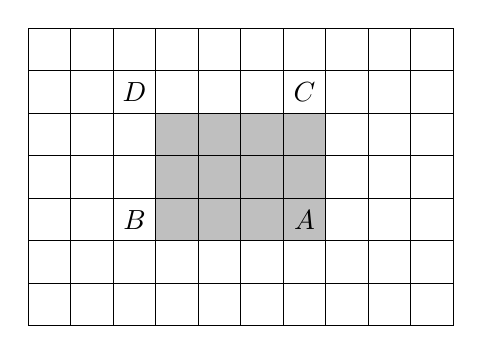
\begin{tikzpicture}[scale=0.54]
\draw[fill=lightgray] (3,2) rectangle (7,5);
\draw (0,0) grid (10,7);
\node[anchor=center] at (6.5, 2.5) {$A$};
\node[anchor=center] at (2.5, 2.5) {$B$};
\node[anchor=center] at (6.5, 5.5) {$C$};
\node[anchor=center] at (2.5, 5.5) {$D$};
\end{tikzpicture}
\end{center}
\end{samepage}

مجموع زیرآرایه خاکستری با فرمول زیر محاسبه می‌شود:
\[S(A) - S(B) - S(C) + S(D),\]
که در آن $S(X)$ بیانگر مجموع مقادیر در زیرآرایه مستطیلی از گوشه بالا سمت چپ تا موقعیت $X$ است.

\subsubsection{پرس‌وجوهای کمینه}

\index{sparse table}

پردازش پرس‌وجوهای کمینه دشوارتر از پرس‌وجوهای مجموع است.
با این حال، روش پیش‌پردازش ساده‌ای با زمان $O(n \log n)$ وجود دارد که پس از آن می‌توان به هر پرس‌وجوی کمینه در زمان $O(1)$ پاسخ داد\footnote{این روش در \cite{ben00} معرفی شد و گاهی روش \key{sparse table} (جدول تنک) نامیده می‌شود.
روش‌های پیچیده‌تری نیز وجود دارند \cite{fis06} که زمان پیش‌پردازش در آن‌ها $O(n)$ است، اما این الگوریتم‌ها در برنامه‌نویسی رقابتی نیاز نیستند.}.
چون پرس‌وجوهای کمینه و بیشینه یکسان پردازش می‌شوند، روی پرس‌وجوهای کمینه تمرکز می‌کنیم.

ایده: پیش‌محاسبه تمام مقادیر $\textrm{min}_q(a,b)$ که در آن‌ها $b-a+1$ (طول بازه) توانی از دو است.
برای نمونه، برای آرایه

\begin{center}
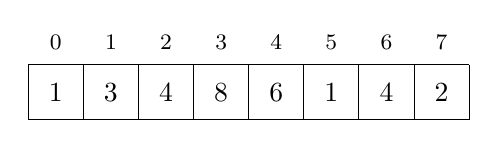
\begin{tikzpicture}[scale=0.7]
\draw (0,0) grid (8,1);

\node at (0.5,0.5) {$1$};
\node at (1.5,0.5) {$3$};
\node at (2.5,0.5) {$4$};
\node at (3.5,0.5) {$8$};
\node at (4.5,0.5) {$6$};
\node at (5.5,0.5) {$1$};
\node at (6.5,0.5) {$4$};
\node at (7.5,0.5) {$2$};

\footnotesize
\node at (0.5,1.4) {$0$};
\node at (1.5,1.4) {$1$};
\node at (2.5,1.4) {$2$};
\node at (3.5,1.4) {$3$};
\node at (4.5,1.4) {$4$};
\node at (5.5,1.4) {$5$};
\node at (6.5,1.4) {$6$};
\node at (7.5,1.4) {$7$};
\end{tikzpicture}
\end{center}
مقادیر زیر محاسبه می‌شوند:

\begin{center}
\begin{tabular}{ccc}

\begin{tabular}{lll}
$a$ & $b$ & $\texttt{min}_q(a,b)$ \\
\hline
0 & 0 & 1 \\
1 & 1 & 3 \\
2 & 2 & 4 \\
3 & 3 & 8 \\
4 & 4 & 6 \\
5 & 5 & 1 \\
6 & 6 & 4 \\
7 & 7 & 2 \\
\end{tabular}

&

\begin{tabular}{lll}
$a$ & $b$ & $\texttt{min}_q(a,b)$ \\
\hline
0 & 1 & 1 \\
1 & 2 & 3 \\
2 & 3 & 4 \\
3 & 4 & 6 \\
4 & 5 & 1 \\
5 & 6 & 1 \\
6 & 7 & 2 \\
\\
\end{tabular}

&

\begin{tabular}{lll}
$a$ & $b$ & $\texttt{min}_q(a,b)$ \\
\hline
0 & 3 & 1 \\
1 & 4 & 3 \\
2 & 5 & 1 \\
3 & 6 & 1 \\
4 & 7 & 1 \\
0 & 7 & 1 \\
\\
\\
\end{tabular}

\end{tabular}
\end{center}

تعداد مقادیر پیش‌محاسبه‌شده $O(n \log n)$ است، زیرا $O(\log n)$ طول بازه توانی از دو داریم.
این مقادیر با فرمول بازگشتی زیر بهینه محاسبه می‌شوند:
\[\texttt{min}_q(a,b) = \min(\texttt{min}_q(a,a+w-1),\texttt{min}_q(a+w,b)),\]
که در آن $b-a+1$ توانی از دو و $w=(b-a+1)/2$ است.
محاسبه همه مقادیر زمان $O(n \log n)$ می‌برد.

پس از این، هر مقدار $\texttt{min}_q(a,b)$ در زمان $O(1)$ به صورت کمینه دو مقدار از پیش محاسبه‌شده به دست می‌آید.
فرض کنید $k$ بزرگ‌ترین توان دو باشد که از $b-a+1$ بیشتر نیست.
می‌توان مقدار $\texttt{min}_q(a,b)$ را با رابطه زیر محاسبه کرد:
\[\texttt{min}_q(a,b) = \min(\texttt{min}_q(a,a+k-1),\texttt{min}_q(b-k+1,b)).\]
در رابطه بالا، بازه $[a,b]$ به صورت اجتماع بازه‌های $[a,a+k-1]$ و $[b-k+1,b]$ نشان داده شده است که طول هر دو $k$ است.

به عنوان مثال، بازه $[1,6]$ را در نظر بگیرید:
\begin{center}
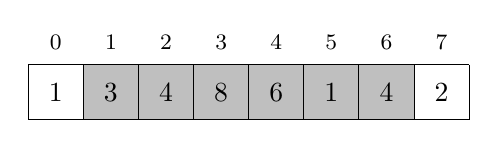
\begin{tikzpicture}[scale=0.7]
\fill[color=lightgray] (1,0) rectangle (7,1);
\draw (0,0) grid (8,1);

\node at (0.5,0.5) {$1$};
\node at (1.5,0.5) {$3$};
\node at (2.5,0.5) {$4$};
\node at (3.5,0.5) {$8$};
\node at (4.5,0.5) {$6$};
\node at (5.5,0.5) {$1$};
\node at (6.5,0.5) {$4$};
\node at (7.5,0.5) {$2$};

\footnotesize
\node at (0.5,1.4) {$0$};
\node at (1.5,1.4) {$1$};
\node at (2.5,1.4) {$2$};
\node at (3.5,1.4) {$3$};
\node at (4.5,1.4) {$4$};
\node at (5.5,1.4) {$5$};
\node at (6.5,1.4) {$6$};
\node at (7.5,1.4) {$7$};
\end{tikzpicture}
\end{center}
طول این بازه ۶ است،
و بزرگ‌ترین توان دو که از ۶ بیشتر نیست ۴ است.
بنابراین بازه $[1,6]$ اجتماع بازه‌های $[1,4]$ و $[3,6]$ است:
\begin{center}
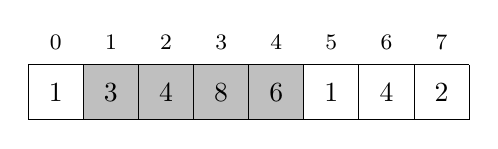
\begin{tikzpicture}[scale=0.7]
\fill[color=lightgray] (1,0) rectangle (5,1);
\draw (0,0) grid (8,1);

\node at (0.5,0.5) {$1$};
\node at (1.5,0.5) {$3$};
\node at (2.5,0.5) {$4$};
\node at (3.5,0.5) {$8$};
\node at (4.5,0.5) {$6$};
\node at (5.5,0.5) {$1$};
\node at (6.5,0.5) {$4$};
\node at (7.5,0.5) {$2$};

\footnotesize
\node at (0.5,1.4) {$0$};
\node at (1.5,1.4) {$1$};
\node at (2.5,1.4) {$2$};
\node at (3.5,1.4) {$3$};
\node at (4.5,1.4) {$4$};
\node at (5.5,1.4) {$5$};
\node at (6.5,1.4) {$6$};
\node at (7.5,1.4) {$7$};
\end{tikzpicture}
\end{center}
\begin{center}
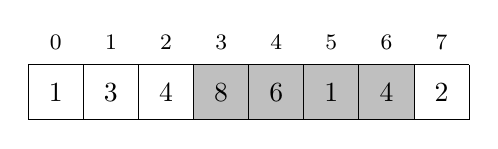
\begin{tikzpicture}[scale=0.7]
\fill[color=lightgray] (3,0) rectangle (7,1);
\draw (0,0) grid (8,1);

\node at (0.5,0.5) {$1$};
\node at (1.5,0.5) {$3$};
\node at (2.5,0.5) {$4$};
\node at (3.5,0.5) {$8$};
\node at (4.5,0.5) {$6$};
\node at (5.5,0.5) {$1$};
\node at (6.5,0.5) {$4$};
\node at (7.5,0.5) {$2$};


\footnotesize
\node at (0.5,1.4) {$0$};
\node at (1.5,1.4) {$1$};
\node at (2.5,1.4) {$2$};
\node at (3.5,1.4) {$3$};
\node at (4.5,1.4) {$4$};
\node at (5.5,1.4) {$5$};
\node at (6.5,1.4) {$6$};
\node at (7.5,1.4) {$7$};
\end{tikzpicture}
\end{center}
از آنجا که $\texttt{min}_q(1,4)=3$ و $\texttt{min}_q(3,6)=1$،
نتیجه می‌گیریم $\texttt{min}_q(1,6)=1$.

\section{درخت ایندکس دودویی}

\index{binary indexed tree}
\index{Fenwick tree}

یک \key{درخت ایندکس دودویی} یا \key{درخت فنویک}\footnote{ساختار داده درخت ایندکس دودویی توسط پی. ام. فنویک در سال ۱۹۹۴ معرفی شد \cite{fen94}.}
را می‌توان نسخه پویای آرایه مجموع پیشوندی دانست.
این ساختار داده از دو عملیات با پیچیدگی زمانی $O(\log n)$ روی آرایه پشتیبانی می‌کند:
پاسخ به پرسش مجموع بازه‌ای و به‌روزرسانی یک مقدار.

مزیت درخت ایندکس‌شده دودویی (فنویک)
امکان به‌روزرسانی کارآمد مقادیر آرایه
بین پرسش‌های مجموع است.
این کار با آرایه مجموع پیشوندی ممکن نیست،
زیرا پس از هر به‌روزرسانی، ساخت دوباره کل آرایه
مجموع پیشوندی در زمان $O(n)$ نیاز است.

\subsubsection{ساختار}

گرچه نام ساختار \emph{درخت} ایندکس‌شده دودویی است،
معمولاً به‌صورت یک آرایه نمایش داده می‌شود.
در این بخش فرض می‌کنیم اندیس آرایه‌ها از یک شروع می‌شود،
زیرا پیاده‌سازی را ساده‌تر می‌کند.

فرض کنید $p(k)$ بزرگ‌ترین توان دو باشد که
$k$ را عاد می‌کند.
درخت ایندکس‌شده دودویی را در آرایه \texttt{tree} ذخیره می‌کنیم
به‌طوری که
\[ \texttt{tree}[k] = \texttt{sum}_q(k-p(k)+1,k),\]
یعنی هر موقعیت $k$ شامل مجموع مقادیر بازه‌ای
از آرایه اصلی با طول $p(k)$ است
که در موقعیت $k$ پایان می‌یابد.
برای نمونه، چون $p(6)=2$ است، $\texttt{tree}[6]$
شامل مقدار $\texttt{sum}_q(5,6)$ است.

برای نمونه، آرایه زیر را در نظر بگیرید:
\begin{center}
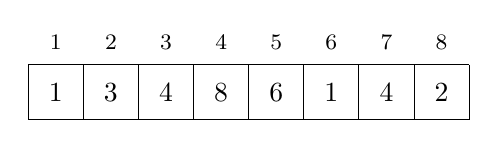
\begin{tikzpicture}[scale=0.7]
\draw (0,0) grid (8,1);

\node at (0.5,0.5) {$1$};
\node at (1.5,0.5) {$3$};
\node at (2.5,0.5) {$4$};
\node at (3.5,0.5) {$8$};
\node at (4.5,0.5) {$6$};
\node at (5.5,0.5) {$1$};
\node at (6.5,0.5) {$4$};
\node at (7.5,0.5) {$2$};

\footnotesize
\node at (0.5,1.4) {$1$};
\node at (1.5,1.4) {$2$};
\node at (2.5,1.4) {$3$};
\node at (3.5,1.4) {$4$};
\node at (4.5,1.4) {$5$};
\node at (5.5,1.4) {$6$};
\node at (6.5,1.4) {$7$};
\node at (7.5,1.4) {$8$};
\end{tikzpicture}
\end{center}

درخت ایندکس‌شده دودویی متناظر به این صورت است:
\begin{center}
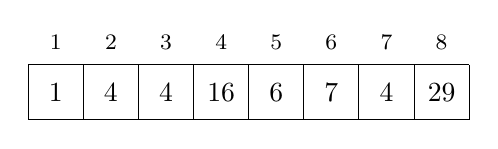
\begin{tikzpicture}[scale=0.7]
\draw (0,0) grid (8,1);

\node at (0.5,0.5) {$1$};
\node at (1.5,0.5) {$4$};
\node at (2.5,0.5) {$4$};
\node at (3.5,0.5) {$16$};
\node at (4.5,0.5) {$6$};
\node at (5.5,0.5) {$7$};
\node at (6.5,0.5) {$4$};
\node at (7.5,0.5) {$29$};

\footnotesize
\node at (0.5,1.4) {$1$};
\node at (1.5,1.4) {$2$};
\node at (2.5,1.4) {$3$};
\node at (3.5,1.4) {$4$};
\node at (4.5,1.4) {$5$};
\node at (5.5,1.4) {$6$};
\node at (6.5,1.4) {$7$};
\node at (7.5,1.4) {$8$};
\end{tikzpicture}
\end{center}

تصویر زیر واضح‌تر نشان می‌دهد که
هر مقدار در درخت ایندکس‌شده دودویی
چگونه با بازه‌ای در آرایه اصلی متناظر است:

\begin{center}
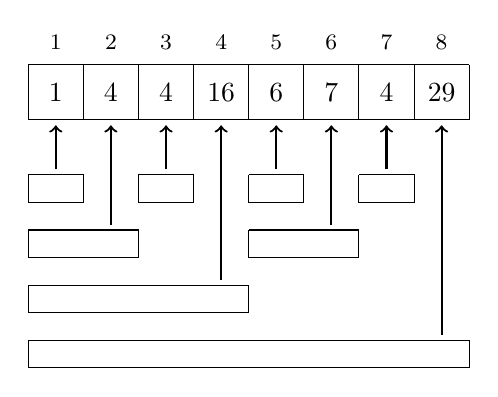
\begin{tikzpicture}[scale=0.7]
\draw (0,0) grid (8,1);

\node at (0.5,0.5) {$1$};
\node at (1.5,0.5) {$4$};
\node at (2.5,0.5) {$4$};
\node at (3.5,0.5) {$16$};
\node at (4.5,0.5) {$6$};
\node at (5.5,0.5) {$7$};
\node at (6.5,0.5) {$4$};
\node at (7.5,0.5) {$29$};

\footnotesize
\node at (0.5,1.4) {$1$};
\node at (1.5,1.4) {$2$};
\node at (2.5,1.4) {$3$};
\node at (3.5,1.4) {$4$};
\node at (4.5,1.4) {$5$};
\node at (5.5,1.4) {$6$};
\node at (6.5,1.4) {$7$};
\node at (7.5,1.4) {$8$};

\draw[->,thick] (0.5,-0.9) -- (0.5,-0.1);
\draw[->,thick] (2.5,-0.9) -- (2.5,-0.1);
\draw[->,thick] (4.5,-0.9) -- (4.5,-0.1);
\draw[->,thick] (6.5,-0.9) -- (6.5,-0.1);
\draw[->,thick] (1.5,-1.9) -- (1.5,-0.1);
\draw[->,thick] (5.5,-1.9) -- (5.5,-0.1);
\draw[->,thick] (3.5,-2.9) -- (3.5,-0.1);
\draw[->,thick] (7.5,-3.9) -- (7.5,-0.1);

\draw (0,-1) -- (1,-1) -- (1,-1.5) -- (0,-1.5) -- (0,-1);
\draw (2,-1) -- (3,-1) -- (3,-1.5) -- (2,-1.5) -- (2,-1);
\draw (4,-1) -- (5,-1) -- (5,-1.5) -- (4,-1.5) -- (4,-1);
\draw (6,-1) -- (7,-1) -- (7,-1.5) -- (6,-1.5) -- (6,-1);
\draw (0,-2) -- (2,-2) -- (2,-2.5) -- (0,-2.5) -- (0,-2);
\draw (4,-2) -- (6,-2) -- (6,-2.5) -- (4,-2.5) -- (4,-2);
\draw (0,-3) -- (4,-3) -- (4,-3.5) -- (0,-3.5) -- (0,-3);
\draw (0,-4) -- (8,-4) -- (8,-4.5) -- (0,-4.5) -- (0,-4);
\end{tikzpicture}
\end{center}

با درخت بندانگشتی دودویی،
هر مقدار $\texttt{sum}_q(1,k)$
در زمان $O(\log n)$ محاسبه می‌شود،
زیرا بازه $[1,k]$ همیشه به
$O(\log n)$ بازه با مجموع ذخیره‌شده در درخت تقسیم‌پذیر است.

برای نمونه، بازه $[1,7]$ شامل
این بازه‌هاست:
\begin{center}
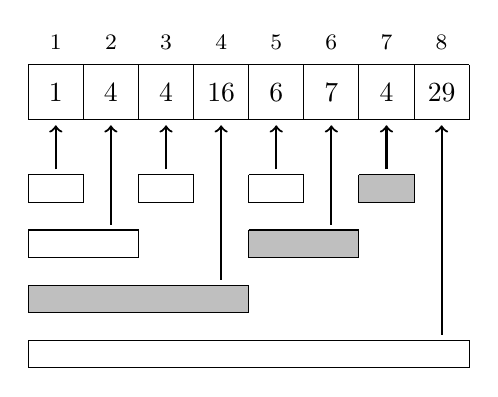
\begin{tikzpicture}[scale=0.7]
\draw (0,0) grid (8,1);

\node at (0.5,0.5) {$1$};
\node at (1.5,0.5) {$4$};
\node at (2.5,0.5) {$4$};
\node at (3.5,0.5) {$16$};
\node at (4.5,0.5) {$6$};
\node at (5.5,0.5) {$7$};
\node at (6.5,0.5) {$4$};
\node at (7.5,0.5) {$29$};

\footnotesize
\node at (0.5,1.4) {$1$};
\node at (1.5,1.4) {$2$};
\node at (2.5,1.4) {$3$};
\node at (3.5,1.4) {$4$};
\node at (4.5,1.4) {$5$};
\node at (5.5,1.4) {$6$};
\node at (6.5,1.4) {$7$};
\node at (7.5,1.4) {$8$};

\draw[->,thick] (0.5,-0.9) -- (0.5,-0.1);
\draw[->,thick] (2.5,-0.9) -- (2.5,-0.1);
\draw[->,thick] (4.5,-0.9) -- (4.5,-0.1);
\draw[->,thick] (6.5,-0.9) -- (6.5,-0.1);
\draw[->,thick] (1.5,-1.9) -- (1.5,-0.1);
\draw[->,thick] (5.5,-1.9) -- (5.5,-0.1);
\draw[->,thick] (3.5,-2.9) -- (3.5,-0.1);
\draw[->,thick] (7.5,-3.9) -- (7.5,-0.1);

\draw (0,-1) -- (1,-1) -- (1,-1.5) -- (0,-1.5) -- (0,-1);
\draw (2,-1) -- (3,-1) -- (3,-1.5) -- (2,-1.5) -- (2,-1);
\draw (4,-1) -- (5,-1) -- (5,-1.5) -- (4,-1.5) -- (4,-1);
\draw[fill=lightgray] (6,-1) -- (7,-1) -- (7,-1.5) -- (6,-1.5) -- (6,-1);
\draw (0,-2) -- (2,-2) -- (2,-2.5) -- (0,-2.5) -- (0,-2);
\draw[fill=lightgray] (4,-2) -- (6,-2) -- (6,-2.5) -- (4,-2.5) -- (4,-2);
\draw[fill=lightgray] (0,-3) -- (4,-3) -- (4,-3.5) -- (0,-3.5) -- (0,-3);
\draw (0,-4) -- (8,-4) -- (8,-4.5) -- (0,-4.5) -- (0,-4);
\end{tikzpicture}
\end{center}
بنابراین مجموع متناظر چنین محاسبه می‌شود:
\[\texttt{sum}_q(1,7)=\texttt{sum}_q(1,4)+\texttt{sum}_q(5,6)+\texttt{sum}_q(7,7)=16+7+4=27\]

برای محاسبه $\texttt{sum}_q(a,b)$ با شرط $a>1$،
همان شگرد آرایه‌های مجموع پیشوندی کار می‌کند:
\[ \texttt{sum}_q(a,b) = \texttt{sum}_q(1,b) - \texttt{sum}_q(1,a-1).\]
محاسبه هر دو عبارت $\texttt{sum}_q(1,b)$
و $\texttt{sum}_q(1,a-1)$ در زمان $O(\log n)$ انجام می‌شود؛
پیچیدگی زمانی کل $O(\log n)$ است.

سپس، پس از به‌روزرسانی مقداری در آرایه اصلی،
چندین مقدار در درخت ایندکس‌شده باینری
باید به‌روزرسانی شوند.
برای مثال، اگر مقدار در جایگاه 3 تغییر کند،
مجموع بازه‌های زیر تغییر می‌کند:
\begin{center}
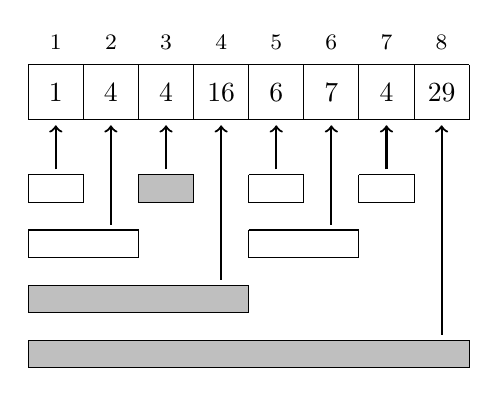
\begin{tikzpicture}[scale=0.7]
\draw (0,0) grid (8,1);

\node at (0.5,0.5) {$1$};
\node at (1.5,0.5) {$4$};
\node at (2.5,0.5) {$4$};
\node at (3.5,0.5) {$16$};
\node at (4.5,0.5) {$6$};
\node at (5.5,0.5) {$7$};
\node at (6.5,0.5) {$4$};
\node at (7.5,0.5) {$29$};

\footnotesize
\node at (0.5,1.4) {$1$};
\node at (1.5,1.4) {$2$};
\node at (2.5,1.4) {$3$};
\node at (3.5,1.4) {$4$};
\node at (4.5,1.4) {$5$};
\node at (5.5,1.4) {$6$};
\node at (6.5,1.4) {$7$};
\node at (7.5,1.4) {$8$};

\draw[->,thick] (0.5,-0.9) -- (0.5,-0.1);
\draw[->,thick] (2.5,-0.9) -- (2.5,-0.1);
\draw[->,thick] (4.5,-0.9) -- (4.5,-0.1);
\draw[->,thick] (6.5,-0.9) -- (6.5,-0.1);
\draw[->,thick] (1.5,-1.9) -- (1.5,-0.1);
\draw[->,thick] (5.5,-1.9) -- (5.5,-0.1);
\draw[->,thick] (3.5,-2.9) -- (3.5,-0.1);
\draw[->,thick] (7.5,-3.9) -- (7.5,-0.1);

\draw (0,-1) -- (1,-1) -- (1,-1.5) -- (0,-1.5) -- (0,-1);
\draw[fill=lightgray] (2,-1) -- (3,-1) -- (3,-1.5) -- (2,-1.5) -- (2,-1);
\draw (4,-1) -- (5,-1) -- (5,-1.5) -- (4,-1.5) -- (4,-1);
\draw (6,-1) -- (7,-1) -- (7,-1.5) -- (6,-1.5) -- (6,-1);
\draw (0,-2) -- (2,-2) -- (2,-2.5) -- (0,-2.5) -- (0,-2);
\draw (4,-2) -- (6,-2) -- (6,-2.5) -- (4,-2.5) -- (4,-2);
\draw[fill=lightgray] (0,-3) -- (4,-3) -- (4,-3.5) -- (0,-3.5) -- (0,-3);
\draw[fill=lightgray] (0,-4) -- (8,-4) -- (8,-4.5) -- (0,-4.5) -- (0,-4);
\end{tikzpicture}
\end{center}

از آنجا که هر عنصر آرایه به $O(\log n)$
بازه در درخت ایندکس‌شده باینری تعلق دارد،
به‌روزرسانی $O(\log n)$ مقدار در درخت کافی است.

\subsubsection{پیاده‌سازی}

عملیات درخت ایندکس‌شده باینری را می‌توان
با استفاده از عملیات بیتی به‌صورت کارا پیاده‌سازی کرد.
نکته کلیدی این است که می‌توانیم
هر مقدار $p(k)$ را با استفاده از فرمول زیر محاسبه کنیم:
\[p(k) = k \& -k.\]

تابع زیر مقدار $\texttt{sum}_q(1,k)$ را محاسبه می‌کند:
\begin{lstlisting}
int sum(int k) {
    int s = 0;
    while (k >= 1) {
        s += tree[k];
        k -= k&-k;
    }
    return s;
}
\end{lstlisting}

تابع زیر مقدار آرایه در جایگاه $k$ را به اندازه $x$ افزایش می‌دهد
($x$ می‌تواند مثبت یا منفی باشد):
\begin{lstlisting}
void add(int k, int x) {
    while (k <= n) {
        tree[k] += x;
        k += k&-k;
    }
}
\end{lstlisting}

پیچیدگی زمانی هر دو تابع
$O(\log n)$ است، زیرا توابع به $O(\log n)$
مقدار در درخت ایندکس‌شده باینری دسترسی دارند، و هر انتقال
به جایگاه بعدی به زمان $O(1)$ نیاز دارد.

\section{درخت بازه‌ای}

\index{segment tree}

یک \key{درخت بازه‌ای}\footnote{پیاده‌سازی پایین‌به‌بالا در این فصل منطبق بر \cite{sta06} است. ساختارهای مشابه در اواخر دهه ۱۹۷۰ برای حل مسائل هندسی استفاده شدند \cite{ben80}.} داده‌ساختاری است که از دو عملیات پشتیبانی می‌کند: پردازش پرس‌وجوی بازه‌ای و به‌روزرسانی مقدار آرایه. درخت‌های بازه‌ای می‌توانند پرس‌وجوهای مجموع، کمینه، بیشینه و بسیاری پرس‌وجوهای دیگر را پشتیبانی کنند به طوری که هر دو عملیات در زمان $O(\log n)$ اجرا شوند.

در مقایسه با درخت اندیس‌گذاری‌شده دودویی، مزیت درخت بازه‌ای عمومی‌تر بودن آن است. در حالی که درخت‌های اندیس‌گذاری‌شده دودویی فقط از پرس‌وجوی مجموع پشتیبانی می‌کنند\footnote{در واقع، با استفاده از \emph{دو} درخت اندیس‌گذاری‌شده دودویی امکان پشتیبانی از پرس‌وجوی کمینه وجود دارد \cite{dim15}، ولی این روش پیچیده‌تر از استفاده از یک درخت بازه‌ای است.}، درخت‌های بازه‌ای پرس‌وجوهای دیگر را نیز پوشش می‌دهند. از سوی دیگر، درخت بازه‌ای حافظه بیشتری مصرف می‌کند و پیاده‌سازی آن کمی دشوارتر است.

\subsubsection{ساختار}

درخت بازه‌ای یک درخت دودویی است که گره‌های سطح پایینی آن متناظر با عناصر آرایه هستند، و گره‌های دیگر حاوی اطلاعات لازم برای پردازش پرس‌وجوهای بازه‌ای می‌باشند.

در این بخش، فرض می‌کنیم اندازه آرایه توانی از دو است و از اندیس‌گذاری بر پایه صفر استفاده می‌شود، زیرا ساخت درخت بازه‌ای برای چنین آرایه‌ای ساده‌تر است. اگر اندازه آرایه توانی از دو نباشد، همیشه می‌توان عناصر اضافی به آن افزود.

ابتدا به بررسی درخت‌های بازه‌ای با پشتیبانی از پرس‌وجوی مجموع می‌پردازیم. به عنوان مثال، آرایه زیر را در نظر بگیرید:
\begin{center}
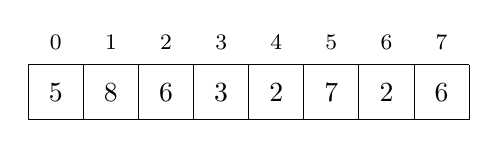
\begin{tikzpicture}[scale=0.7]
\draw (0,0) grid (8,1);

\node at (0.5,0.5) {$5$};
\node at (1.5,0.5) {$8$};
\node at (2.5,0.5) {$6$};
\node at (3.5,0.5) {$3$};
\node at (4.5,0.5) {$2$};
\node at (5.5,0.5) {$7$};
\node at (6.5,0.5) {$2$};
\node at (7.5,0.5) {$6$};

\footnotesize
\node at (0.5,1.4) {$0$};
\node at (1.5,1.4) {$1$};
\node at (2.5,1.4) {$2$};
\node at (3.5,1.4) {$3$};
\node at (4.5,1.4) {$4$};
\node at (5.5,1.4) {$5$};
\node at (6.5,1.4) {$6$};
\node at (7.5,1.4) {$7$};
\end{tikzpicture}
\end{center}
درخت بازه‌ای متناظر به صورت زیر است:
\begin{center}
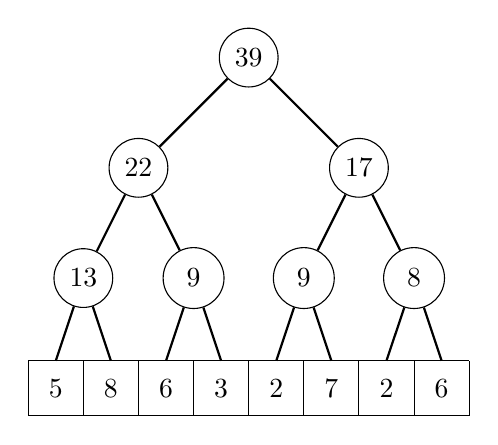
\begin{tikzpicture}[scale=0.7]
\draw (0,0) grid (8,1);

\node[anchor=center] at (0.5, 0.5) {5};
\node[anchor=center] at (1.5, 0.5) {8};
\node[anchor=center] at (2.5, 0.5) {6};
\node[anchor=center] at (3.5, 0.5) {3};
\node[anchor=center] at (4.5, 0.5) {2};
\node[anchor=center] at (5.5, 0.5) {7};
\node[anchor=center] at (6.5, 0.5) {2};
\node[anchor=center] at (7.5, 0.5) {6};

\node[draw, circle] (a) at (1,2.5) {13};
\path[draw,thick,-] (a) -- (0.5,1);
\path[draw,thick,-] (a) -- (1.5,1);
\node[draw, circle,minimum size=22pt] (b) at (3,2.5) {9};
\path[draw,thick,-] (b) -- (2.5,1);
\path[draw,thick,-] (b) -- (3.5,1);
\node[draw, circle,minimum size=22pt] (c) at (5,2.5) {9};
\path[draw,thick,-] (c) -- (4.5,1);
\path[draw,thick,-] (c) -- (5.5,1);
\node[draw, circle,minimum size=22pt] (d) at (7,2.5) {8};
\path[draw,thick,-] (d) -- (6.5,1);
\path[draw,thick,-] (d) -- (7.5,1);

\node[draw, circle] (i) at (2,4.5) {22};
\path[draw,thick,-] (i) -- (a);
\path[draw,thick,-] (i) -- (b);
\node[draw, circle] (j) at (6,4.5) {17};
\path[draw,thick,-] (j) -- (c);
\path[draw,thick,-] (j) -- (d);

\node[draw, circle] (m) at (4,6.5) {39};
\path[draw,thick,-] (m) -- (i);
\path[draw,thick,-] (m) -- (j);
\end{tikzpicture}
\end{center}

هر گره داخلی درخت
متناظر با بازه‌ای از آرایه است
که اندازه‌اش توانی از دو است.
در درخت بالا، مقدار هر گره داخلی
برابر با مجموع مقادیر آرایه مربوطه است
و می‌توان آن را به صورت مجموع مقادیر
گره‌های فرزند چپ و راست محاسبه کرد.

مشخص می‌شود که هر بازه $[a,b]$
را می‌توان به $O(\log n)$ بازه تقسیم کرد
که مقادیر آن‌ها در گره‌های درخت ذخیره شده‌اند.
برای مثال، بازه [2,7] را در نظر بگیرید:
\begin{center}
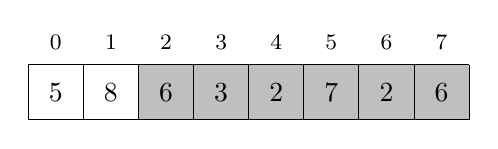
\begin{tikzpicture}[scale=0.7]
\fill[color=gray!50] (2,0) rectangle (8,1);
\draw (0,0) grid (8,1);

\node[anchor=center] at (0.5, 0.5) {5};
\node[anchor=center] at (1.5, 0.5) {8};
\node[anchor=center] at (2.5, 0.5) {6};
\node[anchor=center] at (3.5, 0.5) {3};
\node[anchor=center] at (4.5, 0.5) {2};
\node[anchor=center] at (5.5, 0.5) {7};
\node[anchor=center] at (6.5, 0.5) {2};
\node[anchor=center] at (7.5, 0.5) {6};

\footnotesize
\node at (0.5,1.4) {$0$};
\node at (1.5,1.4) {$1$};
\node at (2.5,1.4) {$2$};
\node at (3.5,1.4) {$3$};
\node at (4.5,1.4) {$4$};
\node at (5.5,1.4) {$5$};
\node at (6.5,1.4) {$6$};
\node at (7.5,1.4) {$7$};
\end{tikzpicture}
\end{center}
در اینجا $\texttt{sum}_q(2,7)=6+3+2+7+2+6=26$.
در این حالت، دو گره زیر در درخت
متناظر با این بازه هستند:
\begin{center}
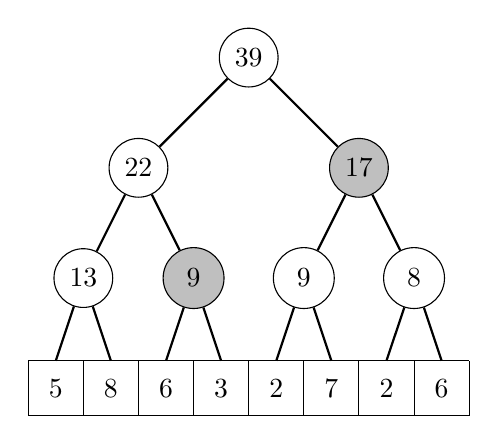
\begin{tikzpicture}[scale=0.7]
\draw (0,0) grid (8,1);

\node[anchor=center] at (0.5, 0.5) {5};
\node[anchor=center] at (1.5, 0.5) {8};
\node[anchor=center] at (2.5, 0.5) {6};
\node[anchor=center] at (3.5, 0.5) {3};
\node[anchor=center] at (4.5, 0.5) {2};
\node[anchor=center] at (5.5, 0.5) {7};
\node[anchor=center] at (6.5, 0.5) {2};
\node[anchor=center] at (7.5, 0.5) {6};

\node[draw, circle] (a) at (1,2.5) {13};
\path[draw,thick,-] (a) -- (0.5,1);
\path[draw,thick,-] (a) -- (1.5,1);
\node[draw, circle,fill=gray!50,minimum size=22pt] (b) at (3,2.5) {9};
\path[draw,thick,-] (b) -- (2.5,1);
\path[draw,thick,-] (b) -- (3.5,1);
\node[draw, circle,minimum size=22pt] (c) at (5,2.5) {9};
\path[draw,thick,-] (c) -- (4.5,1);
\path[draw,thick,-] (c) -- (5.5,1);
\node[draw, circle,minimum size=22pt] (d) at (7,2.5) {8};
\path[draw,thick,-] (d) -- (6.5,1);
\path[draw,thick,-] (d) -- (7.5,1);

\node[draw, circle] (i) at (2,4.5) {22};
\path[draw,thick,-] (i) -- (a);
\path[draw,thick,-] (i) -- (b);
\node[draw, circle,fill=gray!50] (j) at (6,4.5) {17};
\path[draw,thick,-] (j) -- (c);
\path[draw,thick,-] (j) -- (d);

\node[draw, circle] (m) at (4,6.5) {39};
\path[draw,thick,-] (m) -- (i);
\path[draw,thick,-] (m) -- (j);
\end{tikzpicture}
\end{center}
بنابراین، روش دیگر برای محاسبه مجموع $9+17=26$ است.

وقتی مجموع با استفاده از گره‌های تا حد امکان بالا در درخت محاسبه شود، در هر سطح حداکثر دو گره نیاز است. بنابراین، تعداد کل گره‌ها $O(\log n)$ است.

پس از به‌روزرسانی آرایه، باید تمام گره‌هایی که مقدارشان به مقدار به‌روزشده وابسته است را به‌روزرسانی کنیم. این کار با پیمایش مسیر از عنصر به‌روزشده آرایه به گره بالا و به‌روزرسانی گره‌های طول مسیر انجام می‌شود.

تصویر زیر نشان می‌دهد در صورت تغییر مقدار آرایه 7، کدام گره‌های درخت تغییر می‌کنند:

\begin{center}
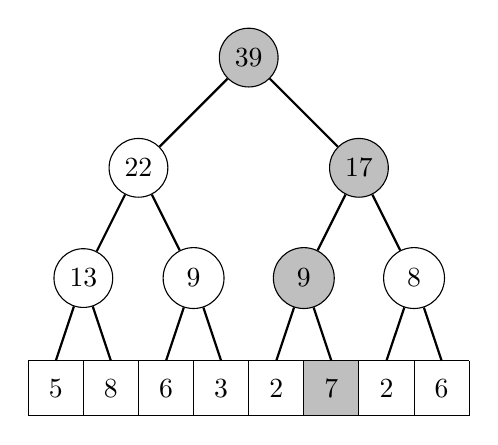
\begin{tikzpicture}[scale=0.7]
\fill[color=gray!50] (5,0) rectangle (6,1);
\draw (0,0) grid (8,1);

\node[anchor=center] at (0.5, 0.5) {5};
\node[anchor=center] at (1.5, 0.5) {8};
\node[anchor=center] at (2.5, 0.5) {6};
\node[anchor=center] at (3.5, 0.5) {3};
\node[anchor=center] at (4.5, 0.5) {2};
\node[anchor=center] at (5.5, 0.5) {7};
\node[anchor=center] at (6.5, 0.5) {2};
\node[anchor=center] at (7.5, 0.5) {6};

\node[draw, circle] (a) at (1,2.5) {13};
\path[draw,thick,-] (a) -- (0.5,1);
\path[draw,thick,-] (a) -- (1.5,1);
\node[draw, circle,minimum size=22pt] (b) at (3,2.5) {9};
\path[draw,thick,-] (b) -- (2.5,1);
\path[draw,thick,-] (b) -- (3.5,1);
\node[draw, circle,minimum size=22pt,fill=gray!50] (c) at (5,2.5) {9};
\path[draw,thick,-] (c) -- (4.5,1);
\path[draw,thick,-] (c) -- (5.5,1);
\node[draw, circle,minimum size=22pt] (d) at (7,2.5) {8};
\path[draw,thick,-] (d) -- (6.5,1);
\path[draw,thick,-] (d) -- (7.5,1);

\node[draw, circle] (i) at (2,4.5) {22};
\path[draw,thick,-] (i) -- (a);
\path[draw,thick,-] (i) -- (b);
\node[draw, circle,fill=gray!50] (j) at (6,4.5) {17};
\path[draw,thick,-] (j) -- (c);
\path[draw,thick,-] (j) -- (d);

\node[draw, circle,fill=gray!50] (m) at (4,6.5) {39};
\path[draw,thick,-] (m) -- (i);
\path[draw,thick,-] (m) -- (j);
\end{tikzpicture}
\end{center}

مسیر از پایین به بالا همیشه شامل $O(\log n)$ گره است، بنابراین هر به‌روزرسانی $O(\log n)$ گره در درخت را تغییر می‌دهد.

\subsubsection{پیاده‌سازی}

درخت بازه‌ای را به عنوان یک آرایه با $2n$ عنصر ذخیره می‌کنیم که $n$ اندازه آرایه اصلی و توانی از دو است. گره‌های درخت از بالا به پایین ذخیره می‌شوند: $\texttt{tree}[1]$ گره ریشه است، $\texttt{tree}[2]$ و $\texttt{tree}[3]$ فرزندان آن هستند و به همین ترتیب. در نهایت، مقادیر از $\texttt{tree}[n]$ تا $\texttt{tree}[2n-1]$ متناظر با مقادیر آرایه اصلی در پایین‌ترین سطح درخت هستند.

برای نمونه، درخت بازه‌ای
\begin{center}
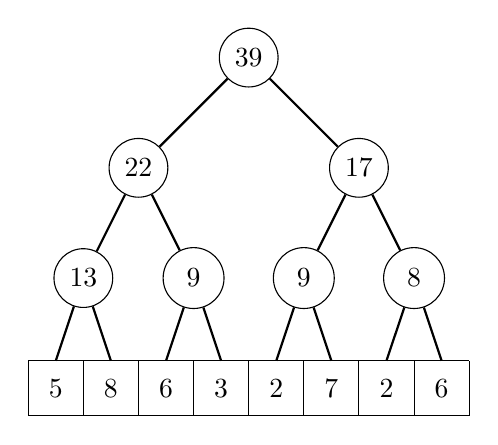
\begin{tikzpicture}[scale=0.7]
\draw (0,0) grid (8,1);

\node[anchor=center] at (0.5, 0.5) {5};
\node[anchor=center] at (1.5, 0.5) {8};
\node[anchor=center] at (2.5, 0.5) {6};
\node[anchor=center] at (3.5, 0.5) {3};
\node[anchor=center] at (4.5, 0.5) {2};
\node[anchor=center] at (5.5, 0.5) {7};
\node[anchor=center] at (6.5, 0.5) {2};
\node[anchor=center] at (7.5, 0.5) {6};

\node[draw, circle] (a) at (1,2.5) {13};
\path[draw,thick,-] (a) -- (0.5,1);
\path[draw,thick,-] (a) -- (1.5,1);
\node[draw, circle,minimum size=22pt] (b) at (3,2.5) {9};
\path[draw,thick,-] (b) -- (2.5,1);
\path[draw,thick,-] (b) -- (3.5,1);
\node[draw, circle,minimum size=22pt] (c) at (5,2.5) {9};
\path[draw,thick,-] (c) -- (4.5,1);
\path[draw,thick,-] (c) -- (5.5,1);
\node[draw, circle,minimum size=22pt] (d) at (7,2.5) {8};
\path[draw,thick,-] (d) -- (6.5,1);
\path[draw,thick,-] (d) -- (7.5,1);

\node[draw, circle] (i) at (2,4.5) {22};
\path[draw,thick,-] (i) -- (a);
\path[draw,thick,-] (i) -- (b);
\node[draw, circle] (j) at (6,4.5) {17};
\path[draw,thick,-] (j) -- (c);
\path[draw,thick,-] (j) -- (d);

\node[draw, circle] (m) at (4,6.5) {39};
\path[draw,thick,-] (m) -- (i);
\path[draw,thick,-] (m) -- (j);
\end{tikzpicture}
\end{center}
به صورت زیر ذخیره می‌شود:
\begin{center}
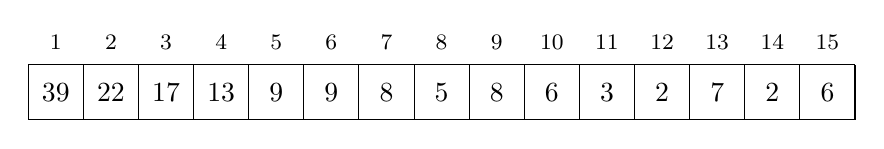
\begin{tikzpicture}[scale=0.7]
\draw (0,0) grid (15,1);

\node at (0.5,0.5) {$39$};
\node at (1.5,0.5) {$22$};
\node at (2.5,0.5) {$17$};
\node at (3.5,0.5) {$13$};
\node at (4.5,0.5) {$9$};
\node at (5.5,0.5) {$9$};
\node at (6.5,0.5) {$8$};
\node at (7.5,0.5) {$5$};
\node at (8.5,0.5) {$8$};
\node at (9.5,0.5) {$6$};
\node at (10.5,0.5) {$3$};
\node at (11.5,0.5) {$2$};
\node at (12.5,0.5) {$7$};
\node at (13.5,0.5) {$2$};
\node at (14.5,0.5) {$6$};

\footnotesize
\node at (0.5,1.4) {$1$};
\node at (1.5,1.4) {$2$};
\node at (2.5,1.4) {$3$};
\node at (3.5,1.4) {$4$};
\node at (4.5,1.4) {$5$};
\node at (5.5,1.4) {$6$};
\node at (6.5,1.4) {$7$};
\node at (7.5,1.4) {$8$};
\node at (8.5,1.4) {$9$};
\node at (9.5,1.4) {$10$};
\node at (10.5,1.4) {$11$};
\node at (11.5,1.4) {$12$};
\node at (12.5,1.4) {$13$};
\node at (13.5,1.4) {$14$};
\node at (14.5,1.4) {$15$};
\end{tikzpicture}
\end{center}
با این نمایش،
والد $\texttt{tree}[k]$
برابر $\texttt{tree}[\lfloor k/2 \rfloor]$
و فرزندان آن $\texttt{tree}[2k]$
و $\texttt{tree}[2k+1]$ هستند.
موقعیت گره فرزند چپ زوج و فرزند راست فرد است.

تابع زیر
مقدار $\texttt{sum}_q(a,b)$ را محاسبه می‌کند:
\begin{lstlisting}
int sum(int a, int b) {
    a += n; b += n;
    int s = 0;
    while (a <= b) {
        if (a%2 == 1) s += tree[a++];
        if (b%2 == 0) s += tree[b--];
        a /= 2; b /= 2;
    }
    return s;
}
\end{lstlisting}
تابع بازه‌ای را نگه می‌دارد
که در ابتدا $[a+n,b+n]$ است.
سپس در هر مرحله، بازه یک سطح در درخت بالا می‌رود
و قبل از آن، مقادیر گره‌هایی که به بازه بالاتر
تعلق ندارند به مجموع اضافه می‌شوند.

تابع زیر مقدار آرایه را در موقعیت $k$ به اندازه $x$ افزایش می‌دهد:
\begin{lstlisting}
void add(int k, int x) {
    k += n;
    tree[k] += x;
    for (k /= 2; k >= 1; k /= 2) {
        tree[k] = tree[2*k]+tree[2*k+1];
    }
}
\end{lstlisting}
ابتدا تابع مقدار را در پایین‌ترین سطح درخت به‌روزرسانی می‌کند.
سپس، مقادیر تمام گره‌های داخلی درخت را تا رسیدن به بالاترین گره درخت به‌روز می‌کند.

هر دو تابع بالا در زمان $O(\log n)$ کار می‌کنند، زیرا یک درخت بازه‌ای با $n$ عنصر از $O(\log n)$ سطح تشکیل شده است، و توابع در هر مرحله یک سطح در درخت بالا می‌روند.

\subsubsection{سایر پرس‌وجوها}

درخت‌های بازه‌ای می‌توانند از تمام پرس‌وجوهای بازه‌ای پشتیبانی کنند که در آن‌ها تقسیم بازه به دو بخش، محاسبه پاسخ به‌طور جداگانه برای هر دو بخش، و سپس ترکیب کارآمد پاسخ‌ها امکان‌پذیر باشد.
نمونه‌هایی از این پرس‌وجوها عبارتند از کمینه و بیشینه، بزرگ‌ترین مقسوم‌علیه مشترک، و عملگرهای بیتی and، or و xor.

به عنوان مثال، درخت بازه‌ای زیر از پرس‌وجوهای کمینه پشتیبانی می‌کند:

\begin{center}
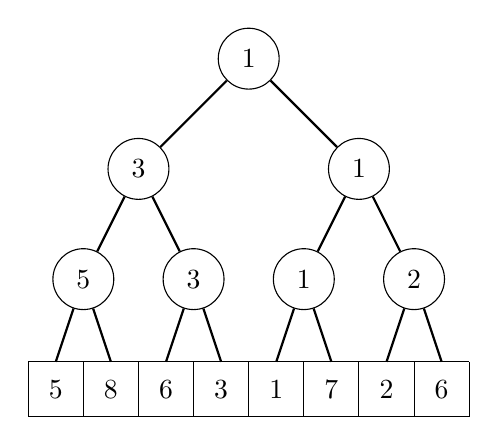
\begin{tikzpicture}[scale=0.7]
\draw (0,0) grid (8,1);

\node[anchor=center] at (0.5, 0.5) {5};
\node[anchor=center] at (1.5, 0.5) {8};
\node[anchor=center] at (2.5, 0.5) {6};
\node[anchor=center] at (3.5, 0.5) {3};
\node[anchor=center] at (4.5, 0.5) {1};
\node[anchor=center] at (5.5, 0.5) {7};
\node[anchor=center] at (6.5, 0.5) {2};
\node[anchor=center] at (7.5, 0.5) {6};

\node[draw, circle,minimum size=22pt] (a) at (1,2.5) {5};
\path[draw,thick,-] (a) -- (0.5,1);
\path[draw,thick,-] (a) -- (1.5,1);
\node[draw, circle,minimum size=22pt] (b) at (3,2.5) {3};
\path[draw,thick,-] (b) -- (2.5,1);
\path[draw,thick,-] (b) -- (3.5,1);
\node[draw, circle,minimum size=22pt] (c) at (5,2.5) {1};
\path[draw,thick,-] (c) -- (4.5,1);
\path[draw,thick,-] (c) -- (5.5,1);
\node[draw, circle,minimum size=22pt] (d) at (7,2.5) {2};
\path[draw,thick,-] (d) -- (6.5,1);
\path[draw,thick,-] (d) -- (7.5,1);

\node[draw, circle,minimum size=22pt] (i) at (2,4.5) {3};
\path[draw,thick,-] (i) -- (a);
\path[draw,thick,-] (i) -- (b);
\node[draw, circle,minimum size=22pt] (j) at (6,4.5) {1};
\path[draw,thick,-] (j) -- (c);
\path[draw,thick,-] (j) -- (d);

\node[draw, circle,minimum size=22pt] (m) at (4,6.5) {1};
\path[draw,thick,-] (m) -- (i);
\path[draw,thick,-] (m) -- (j);
\end{tikzpicture}
\end{center}

در این حالت، هر گره درخت شامل کوچک‌ترین مقدار در بازه متناظر از آرایه است.
بالاترین گره درخت شامل کوچک‌ترین مقدار کل آرایه است.
عملیات را می‌توان مشابه قبل پیاده‌سازی کرد، اما به جای مجموع، کمینه‌ها محاسبه می‌شوند.

ساختار درخت بازه‌ای همچنین امکان استفاده از جستجوی دودویی برای یافتن موقعیت عناصر آرایه را فراهم می‌کند.
به عنوان مثال، اگر درخت از پرس‌وجوهای کمینه پشتیبانی کند، می‌توان موقعیت عنصری با کمترین مقدار را در زمان $O(\log n)$ پیدا کرد.

به عنوان نمونه، در درخت بالا، عنصری با کمترین مقدار ۱ را می‌توان با پیمایش مسیری رو به پایین از بالاترین گره پیدا کرد:

\begin{center}
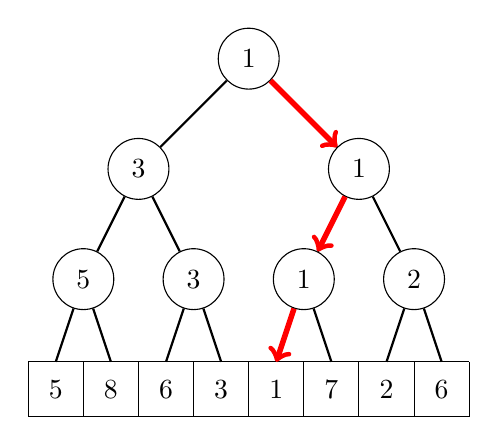
\begin{tikzpicture}[scale=0.7]
\draw (0,0) grid (8,1);

\node[anchor=center] at (0.5, 0.5) {5};
\node[anchor=center] at (1.5, 0.5) {8};
\node[anchor=center] at (2.5, 0.5) {6};
\node[anchor=center] at (3.5, 0.5) {3};
\node[anchor=center] at (4.5, 0.5) {1};
\node[anchor=center] at (5.5, 0.5) {7};
\node[anchor=center] at (6.5, 0.5) {2};
\node[anchor=center] at (7.5, 0.5) {6};

\node[draw, circle,minimum size=22pt] (a) at (1,2.5) {5};
\path[draw,thick,-] (a) -- (0.5,1);
\path[draw,thick,-] (a) -- (1.5,1);
\node[draw, circle,minimum size=22pt] (b) at (3,2.5) {3};
\path[draw,thick,-] (b) -- (2.5,1);
\path[draw,thick,-] (b) -- (3.5,1);
\node[draw, circle,minimum size=22pt] (c) at (5,2.5) {1};
\path[draw,thick,-] (c) -- (4.5,1);
\path[draw,thick,-] (c) -- (5.5,1);
\node[draw, circle,minimum size=22pt] (d) at (7,2.5) {2};
\path[draw,thick,-] (d) -- (6.5,1);
\path[draw,thick,-] (d) -- (7.5,1);

\node[draw, circle,minimum size=22pt] (i) at (2,4.5) {3};
\path[draw,thick,-] (i) -- (a);
\path[draw,thick,-] (i) -- (b);
\node[draw, circle,minimum size=22pt] (j) at (6,4.5) {1};
\path[draw,thick,-] (j) -- (c);
\path[draw,thick,-] (j) -- (d);

\node[draw, circle,minimum size=22pt] (m) at (4,6.5) {1};
\path[draw,thick,-] (m) -- (i);
\path[draw,thick,-] (m) -- (j);

\path[draw=red,thick,->,line width=2pt] (m) -- (j);
\path[draw=red,thick,->,line width=2pt] (j) -- (c);
\path[draw=red,thick,->,line width=2pt] (c) -- (4.5,1);
\end{tikzpicture}
\end{center}

\section{تکنیک‌های تکمیلی}

\subsubsection{فشرده‌سازی اندیس‌ها}

محدودیت ساختارهای داده مبتنی بر آرایه:
اندیس‌ها اعداد صحیح متوالی هستند.
اندیس‌های بزرگ مشکل می‌سازند.
مثال: برای اندیس $10^9$،
آرایه باید $10^9$ عنصر داشته باشد؛
حافظه زیادی هدر می‌رود.

\index{index compression}

راه‌حل: استفاده از \key{فشرده‌سازی اندیس‌ها}.
جایگزینی اندیس‌های اصلی با اندیس‌های $1,2,3,$ و غیره.
شرط اجرا: آگاهی قبلی از تمام اندیس‌های موردنیاز الگوریتم.

ایده: تبدیل هر اندیس اصلی $x$ به $c(x)$ با تابع فشرده‌ساز $c$.
شرط حفظ ترتیب: اگر $a<b$ باشد، باید $c(a)<c(b)$ بماند.
پرس‌وجوها روی اندیس‌های فشرده‌شده نیز کار می‌کنند.

مثال: برای اندیس‌های اصلی $555$، $10^9$ و $8$، اندیس‌های جدید:

\[
\begin{array}{lcl}
c(8) & = & 1 \\
c(555) & = & 2 \\
c(10^9) & = & 3 \\
\end{array}
\]

\subsubsection{به‌روزرسانی‌های بازه‌ای}

تا اینجا: ساختارهای داده با پرس‌وجوی بازه‌ای و به‌روزرسانی تک‌عنصری.
حالت معکوس: به‌روزرسانی بازه‌ها و دریافت مقدار تک‌عنصرها.
عملیات هدف: افزایش تمام عناصر بازه $[a,b]$ به مقدار $x$.

\index{difference array}

در کمال شگفتی، داده‌ساختارهای ارائه‌شده در این فصل در این وضعیت نیز قابل استفاده هستند. برای این کار، یک \key{آرایه تفاضلی} (difference array) می‌سازیم که مقادیر آن نشان‌دهنده تفاضل بین مقادیر متوالی در آرایه اصلی است. بنابراین، آرایه اصلی همان آرایه مجموع پیشوندی آرایه تفاضلی است. برای مثال، آرایه زیر را در نظر بگیرید:

\begin{center}
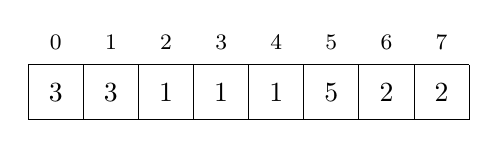
\begin{tikzpicture}[scale=0.7]
\draw (0,0) grid (8,1);

\node at (0.5,0.5) {$3$};
\node at (1.5,0.5) {$3$};
\node at (2.5,0.5) {$1$};
\node at (3.5,0.5) {$1$};
\node at (4.5,0.5) {$1$};
\node at (5.5,0.5) {$5$};
\node at (6.5,0.5) {$2$};
\node at (7.5,0.5) {$2$};


\footnotesize
\node at (0.5,1.4) {$0$};
\node at (1.5,1.4) {$1$};
\node at (2.5,1.4) {$2$};
\node at (3.5,1.4) {$3$};
\node at (4.5,1.4) {$4$};
\node at (5.5,1.4) {$5$};
\node at (6.5,1.4) {$6$};
\node at (7.5,1.4) {$7$};
\end{tikzpicture}
\end{center}

آرایه تفاضلی برای آرایه بالا به صورت زیر است:
\begin{center}
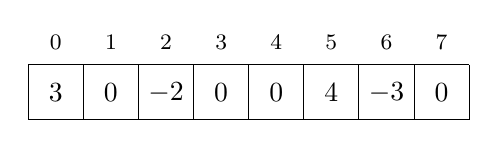
\begin{tikzpicture}[scale=0.7]
\draw (0,0) grid (8,1);

\node at (0.5,0.5) {$3$};
\node at (1.5,0.5) {$0$};
\node at (2.5,0.5) {$-2$};
\node at (3.5,0.5) {$0$};
\node at (4.5,0.5) {$0$};
\node at (5.5,0.5) {$4$};
\node at (6.5,0.5) {$-3$};
\node at (7.5,0.5) {$0$};


\footnotesize
\node at (0.5,1.4) {$0$};
\node at (1.5,1.4) {$1$};
\node at (2.5,1.4) {$2$};
\node at (3.5,1.4) {$3$};
\node at (4.5,1.4) {$4$};
\node at (5.5,1.4) {$5$};
\node at (6.5,1.4) {$6$};
\node at (7.5,1.4) {$7$};
\end{tikzpicture}
\end{center}

برای نمونه، مقدار ۲ در موقعیت ۶ آرایه اصلی متناظر با مجموع $3-2+4-3=2$ در آرایه تفاضلی است.

مزیت آرایه تفاضلی این است که می‌توان یک بازه در آرایه اصلی را صرفاً با تغییر دو عنصر در آرایه تفاضلی به‌روزرسانی کرد. به عنوان مثال، اگر بخواهیم مقادیر آرایه اصلی بین موقعیت‌های ۱ تا ۴ را به اندازه ۵ واحد افزایش دهیم، کافی است مقدار آرایه تفاضلی در موقعیت ۱ را ۵ واحد افزایش داده و مقدار در موقعیت ۵ را ۵ واحد کاهش دهیم. نتیجه به صورت زیر خواهد بود:

\begin{center}
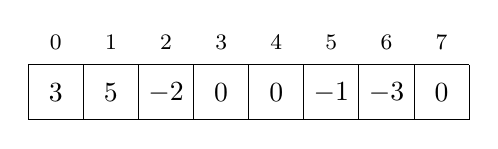
\begin{tikzpicture}[scale=0.7]
\draw (0,0) grid (8,1);

\node at (0.5,0.5) {$3$};
\node at (1.5,0.5) {$5$};
\node at (2.5,0.5) {$-2$};
\node at (3.5,0.5) {$0$};
\node at (4.5,0.5) {$0$};
\node at (5.5,0.5) {$-1$};
\node at (6.5,0.5) {$-3$};
\node at (7.5,0.5) {$0$};

\footnotesize
\node at (0.5,1.4) {$0$};
\node at (1.5,1.4) {$1$};
\node at (2.5,1.4) {$2$};
\node at (3.5,1.4) {$3$};
\node at (4.5,1.4) {$4$};
\node at (5.5,1.4) {$5$};
\node at (6.5,1.4) {$6$};
\node at (7.5,1.4) {$7$};
\end{tikzpicture}
\end{center}

به طور کلی‌تر، برای افزایش مقادیر در بازه $[a,b]$ به اندازه $x$، مقدار در موقعیت $a$ را $x$ واحد افزایش داده و مقدار در موقعیت $b+1$ را $x$ واحد کاهش می‌دهیم. بدین ترتیب تنها نیاز به به‌روزرسانی مقادیر تکی و پردازش پرس‌وجوهای مجموع است، بنابراین می‌توان از درخت اندیس‌گذاری‌شده دودویی یا درخت بازه‌ای استفاده کرد.

مسئله دشوارتر، پشتیبانی هم‌زمان از پرس‌وجوهای بازه‌ای و به‌روزرسانی‌های بازه‌ای است. در فصل ۲۸ خواهیم دید که حتی این کار نیز امکان‌پذیر است.